\section{Results}
We ran the full system for \NumDays{} simulated days (about \RunMinutes{} real minutes) on a MacBook with an
Apple M-series chip and 8\,GB of memory. This section shows what the system produced.

\subsection{Live operations (speed layer)}
Figure~\ref{fig:live} shows the top of the live Grafana dashboard. \LiveText{} The map shows each vehicle
by status (green on a trip, blue going to a pickup, orange idle). The charts show fares by pickup zone, trips
per simulated hour and the status of vehicles in each zone. Further down, the dashboard has a utilisation
heatmap by zone and hour, the open idle alerts and the profit projection for today, which is the Lambda
merge of Section~\ref{sec:serving}.

\begin{figure}[!htb]
\centering
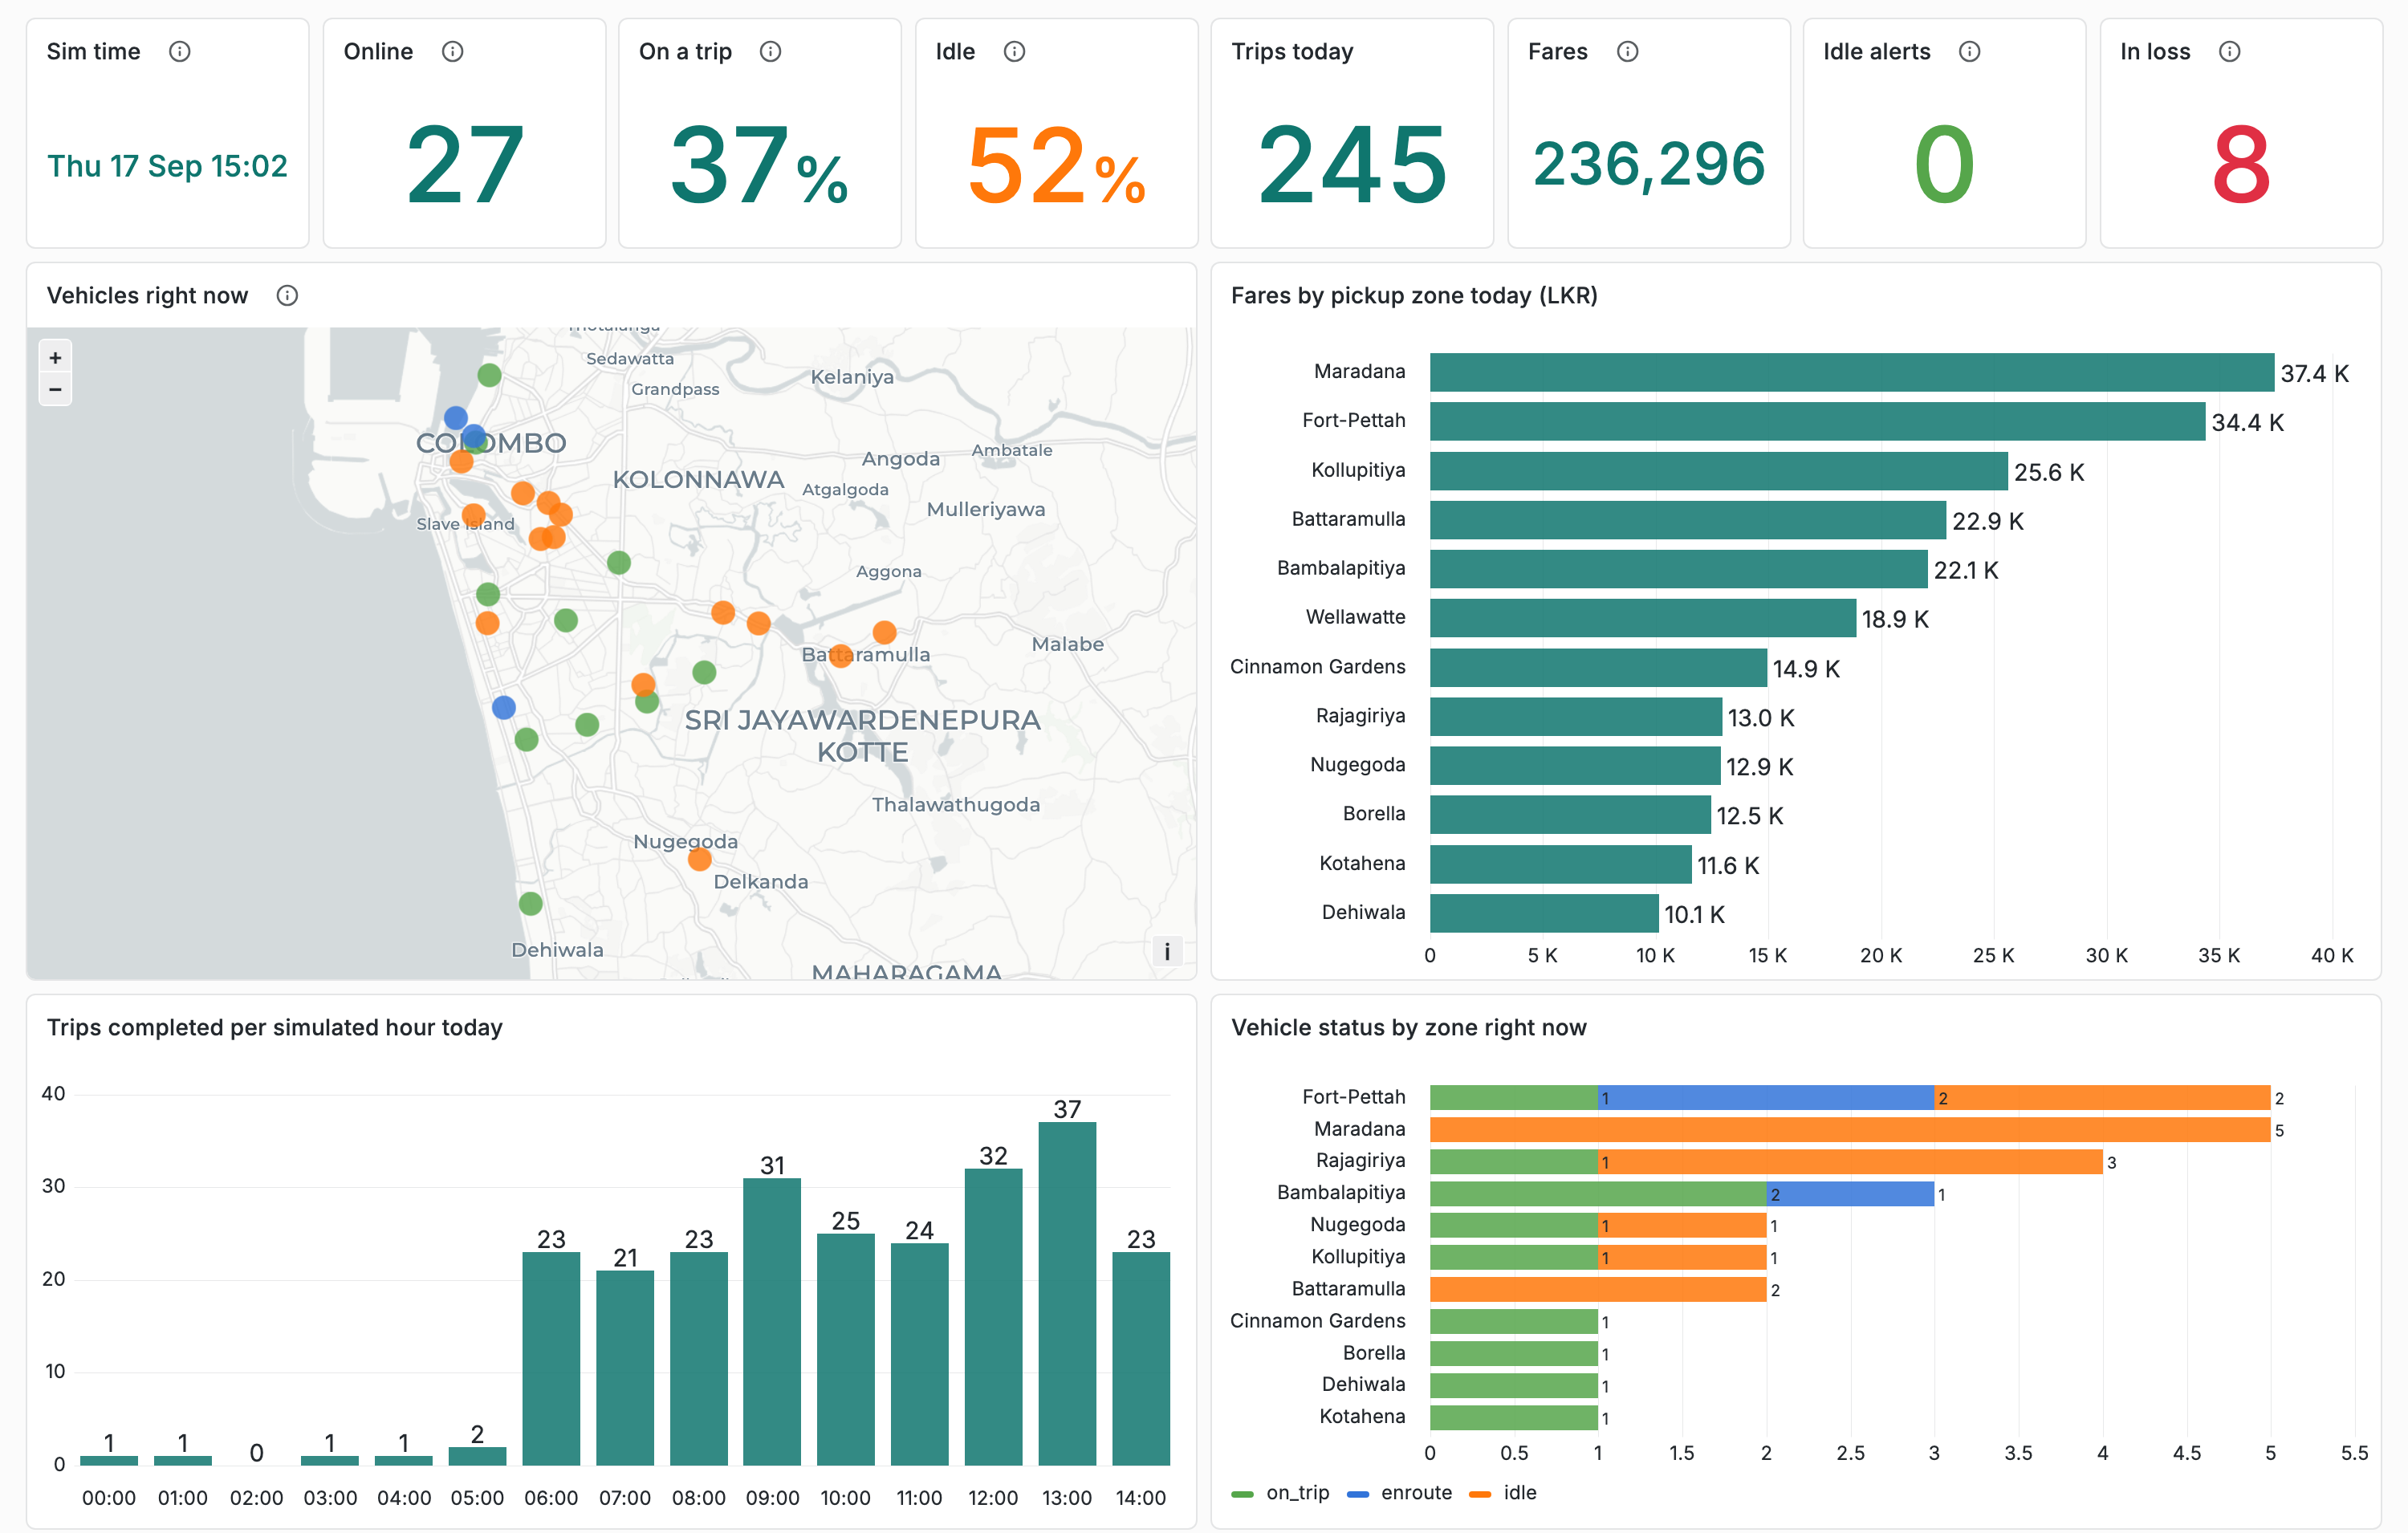
\includegraphics[width=0.92\textwidth]{figures/grafana_live.png}
\caption{Grafana dashboard ``Fleet operations (live)'', fed by the speed layer. It answers the first part of
the business question: utilisation and earnings by area and time of day, right now.}
\label{fig:live}
\end{figure}

\subsection{Daily profitability (batch layer)}
\label{sec:daily}
Table~\ref{tab:daily} gives the exact batch results for each day. Figure~\ref{fig:report} shows the top of
a daily report, and Figure~\ref{fig:trend} shows the daily net profit of the three problem vehicles compared
with the fleet average.

\begin{table}[!htb]
\centering\small
\caption{Exact daily results from the batch layer (money in LKR). Day 1 is 18 hours long.}
\label{tab:daily}
\begin{tabular}{@{}lrrrrrrrr@{}}
\toprule
\textbf{Day} & \textbf{Trips} & \textbf{Fares} & \textbf{Fuel + maint.} & \textbf{Net profit} & \textbf{Util. \%} & \textbf{Unprof.} & \textbf{At risk} & \textbf{Becoming} \\
\midrule
1 Sep & 489 & 483,550 & 154,962 & 183,523 & 41.6 & 0 & 2 & 0 \\
2 Sep & 506 & 497,098 & 155,046 & 192,923 & 42.2 & 1 & 0 & 0 \\
3 Sep & 461 & 451,097 & 159,128 & 156,640 & 39.4 & 2 & 0 & 1 \\
4 Sep & 467 & 455,089 & 187,856 & 130,707 & 39.0 & 4 & 1 & 0 \\
5 Sep & 434 & 438,988 & 155,254 & 152,037 & 38.3 & 4 & 0 & 1 \\
6 Sep & 459 & 464,670 & 193,060 & 132,209 & 40.4 & 3 & 1 & 0 \\
7 Sep & 451 & 443,800 & 167,604 & 143,056 & 39.4 & 3 & 0 & 0 \\
8 Sep & 472 & 453,180 & 181,166 & 136,060 & 38.7 & 3 & 1 & 1 \\
9 Sep & 447 & 443,783 & 197,836 & 112,812 & 38.6 & 6 & 1 & 0 \\
10 Sep & 466 & 462,885 & 152,639 & 171,381 & 39.5 & 2 & 0 & 0 \\
11 Sep & 457 & 456,118 & 154,960 & 164,323 & 40.0 & 2 & 0 & 1 \\
12 Sep & 469 & 469,820 & 170,924 & 157,950 & 40.7 & 3 & 0 & 1 \\
13 Sep & 467 & 457,249 & 175,066 & 145,009 & 39.0 & 2 & 1 & 1 \\
14 Sep & 454 & 442,848 & 159,057 & 150,937 & 38.0 & 3 & 0 & 2 \\
15 Sep & 470 & 462,878 & 194,604 & 129,411 & 39.5 & 5 & 0 & 1 \\
\bottomrule
\end{tabular}
\end{table}


\BusinessText{}

\begin{figure}[!htb]
\centering
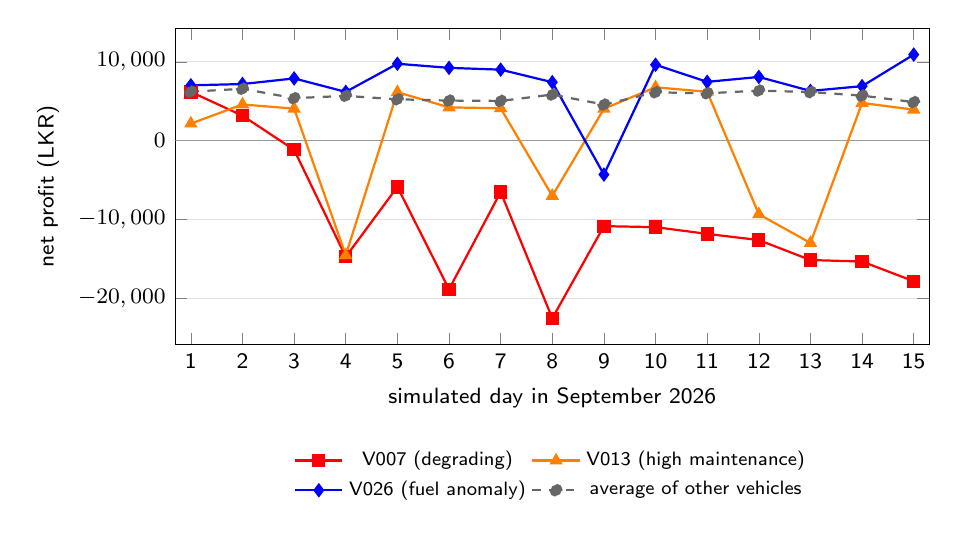
\begin{tikzpicture}
\begin{axis}[width=0.92\textwidth, height=5.6cm, font=\sffamily\footnotesize,
  xtick={1,2,3,4,5,6,7,8,9,10,11,12,13,14,15}, xticklabels={1,2,3,4,5,6,7,8,9,10,11,12,13,14,15}, xmin=0.7, xmax=15.3,
  xlabel={simulated day in September 2026}, ylabel={net profit (LKR)}, ymajorgrids, grid style={black!12},
  yticklabel style={/pgf/number format/fixed, /pgf/number format/1000 sep={,}},
  scaled y ticks=false, legend style={font=\sffamily\scriptsize, at={(0.5,-0.3)}, anchor=north,
  legend columns=2, draw=none}]
\addplot[black!40, thin, forget plot] coordinates {(0.7,0) (15.3,0)};
\addplot[red, mark=square*, thick] coordinates {(1,6199) (2,3182) (3,-1157) (4,-14735) (5,-5858) (6,-18855) (7,-6512) (8,-22536) (9,-10842) (10,-10968) (11,-11826) (12,-12607) (13,-15145) (14,-15331) (15,-17830)};
\addlegendentry{V007 (degrading)}
\addplot[orange, mark=triangle*, thick] coordinates {(1,2176) (2,4601) (3,4073) (4,-14521) (5,6169) (6,4232) (7,4119) (8,-7005) (9,4059) (10,6783) (11,6212) (12,-9324) (13,-12975) (14,4795) (15,3947)};
\addlegendentry{V013 (high maintenance)}
\addplot[blue, mark=diamond*, thick] coordinates {(1,7033) (2,7196) (3,7909) (4,6201) (5,9771) (6,9249) (7,9023) (8,7427) (9,-4294) (10,9641) (11,7474) (12,8095) (13,6323) (14,6928) (15,10933)};
\addlegendentry{V026 (fuel anomaly)}
\addplot[black!60, dashed, thick, mark=*] coordinates {(1,6226) (2,6591) (3,5401) (4,5695) (5,5258) (6,5096) (7,5053) (8,5858) (9,4588) (10,6145) (11,6017) (12,6362) (13,6178) (14,5724) (15,4902)};
\addlegendentry{average of other vehicles}
\end{axis}
\end{tikzpicture}

\caption{Daily net profit of the vehicles with special profiles and the average of all other vehicles
(batch layer, LKR).}
\label{fig:trend}
\end{figure}

\begin{figure}[!htb]
\centering
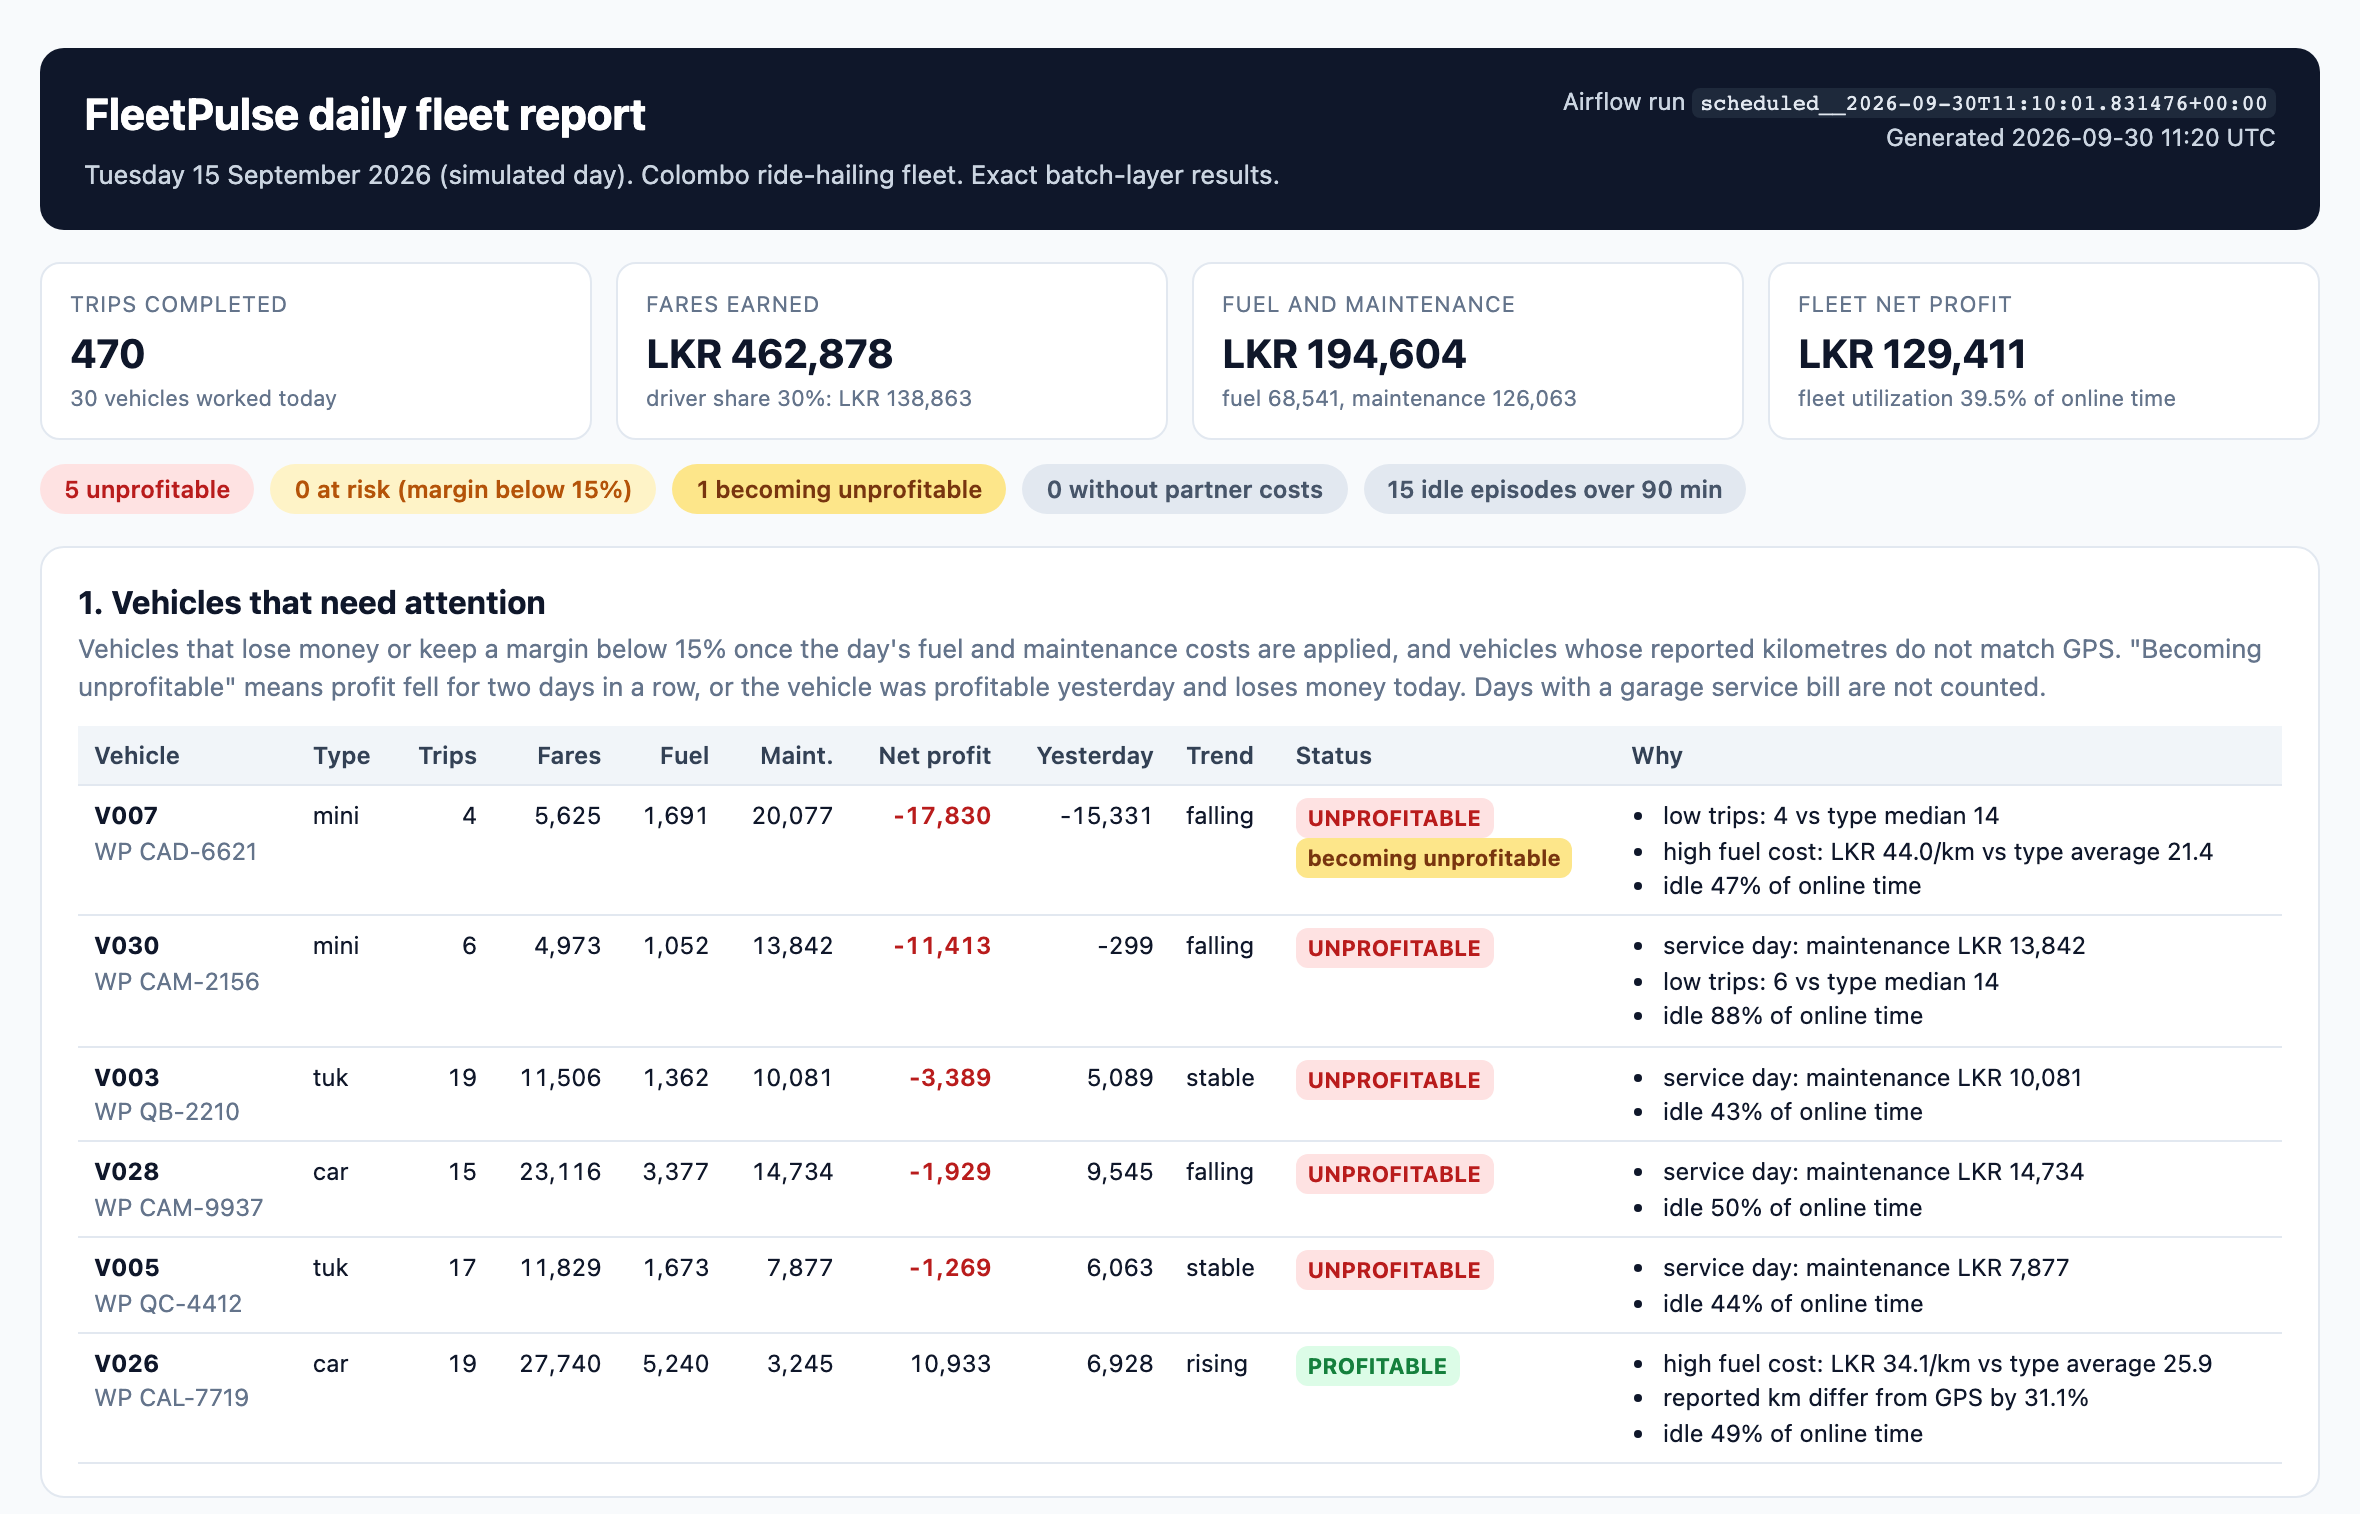
\includegraphics[width=0.86\textwidth]{figures/daily_report_top.png}
\caption{Top of the daily HTML report built by Airflow for day \ReportDay{}. It lists the vehicles that
need attention and explains why, which answers the second part of the business question.}
\label{fig:report}
\end{figure}

\subsection{Speed layer compared with the batch layer}
\label{sec:reconciliation}
After each batch run the DAG compares the day's totals from both layers (Table~\ref{tab:recon}). The speed
layer missed some events because they arrived after its 10-minute watermark. The batch layer read the
complete day, so it recovered them. \ReconText{}

\begin{table}[!htb]
\centering\small
\caption{Speed layer compared with the batch layer, and what the batch layer cleaned, per day (days 2 to 15, lowest, average and highest day).}
\label{tab:recon}
\begin{tabularx}{\textwidth}{@{}L rrr@{}}
\toprule
\textbf{Measure per day} & \textbf{Lowest} & \textbf{Average} & \textbf{Highest} \\
\midrule
Trips missed by the speed layer & 0 & 1.9 & 5 \\
Fares missed by the speed layer (\% of batch fares) & 0.00 & 0.42 & 1.11 \\
Pings missed by the speed layer (\% of batch pings) & 0.08 & 0.31 & 0.66 \\
Late events (more than 10 simulated minutes) & 55 & 174 & 256 \\
Repeated events removed & 84 & 109 & 134 \\
Invalid events removed & 24 & 35 & 47 \\
Bad cost rows put in quarantine & 0 & 1.6 & 3 \\
\bottomrule
\end{tabularx}
\end{table}


\subsection{Orchestration and pipeline health}
Figure~\ref{fig:dag} in Section~\ref{sec:batch} shows the Airflow runs, and Figure~\ref{fig:health} shows the pipeline
health dashboard. \HealthText{}

\begin{figure}[!htb]
\centering
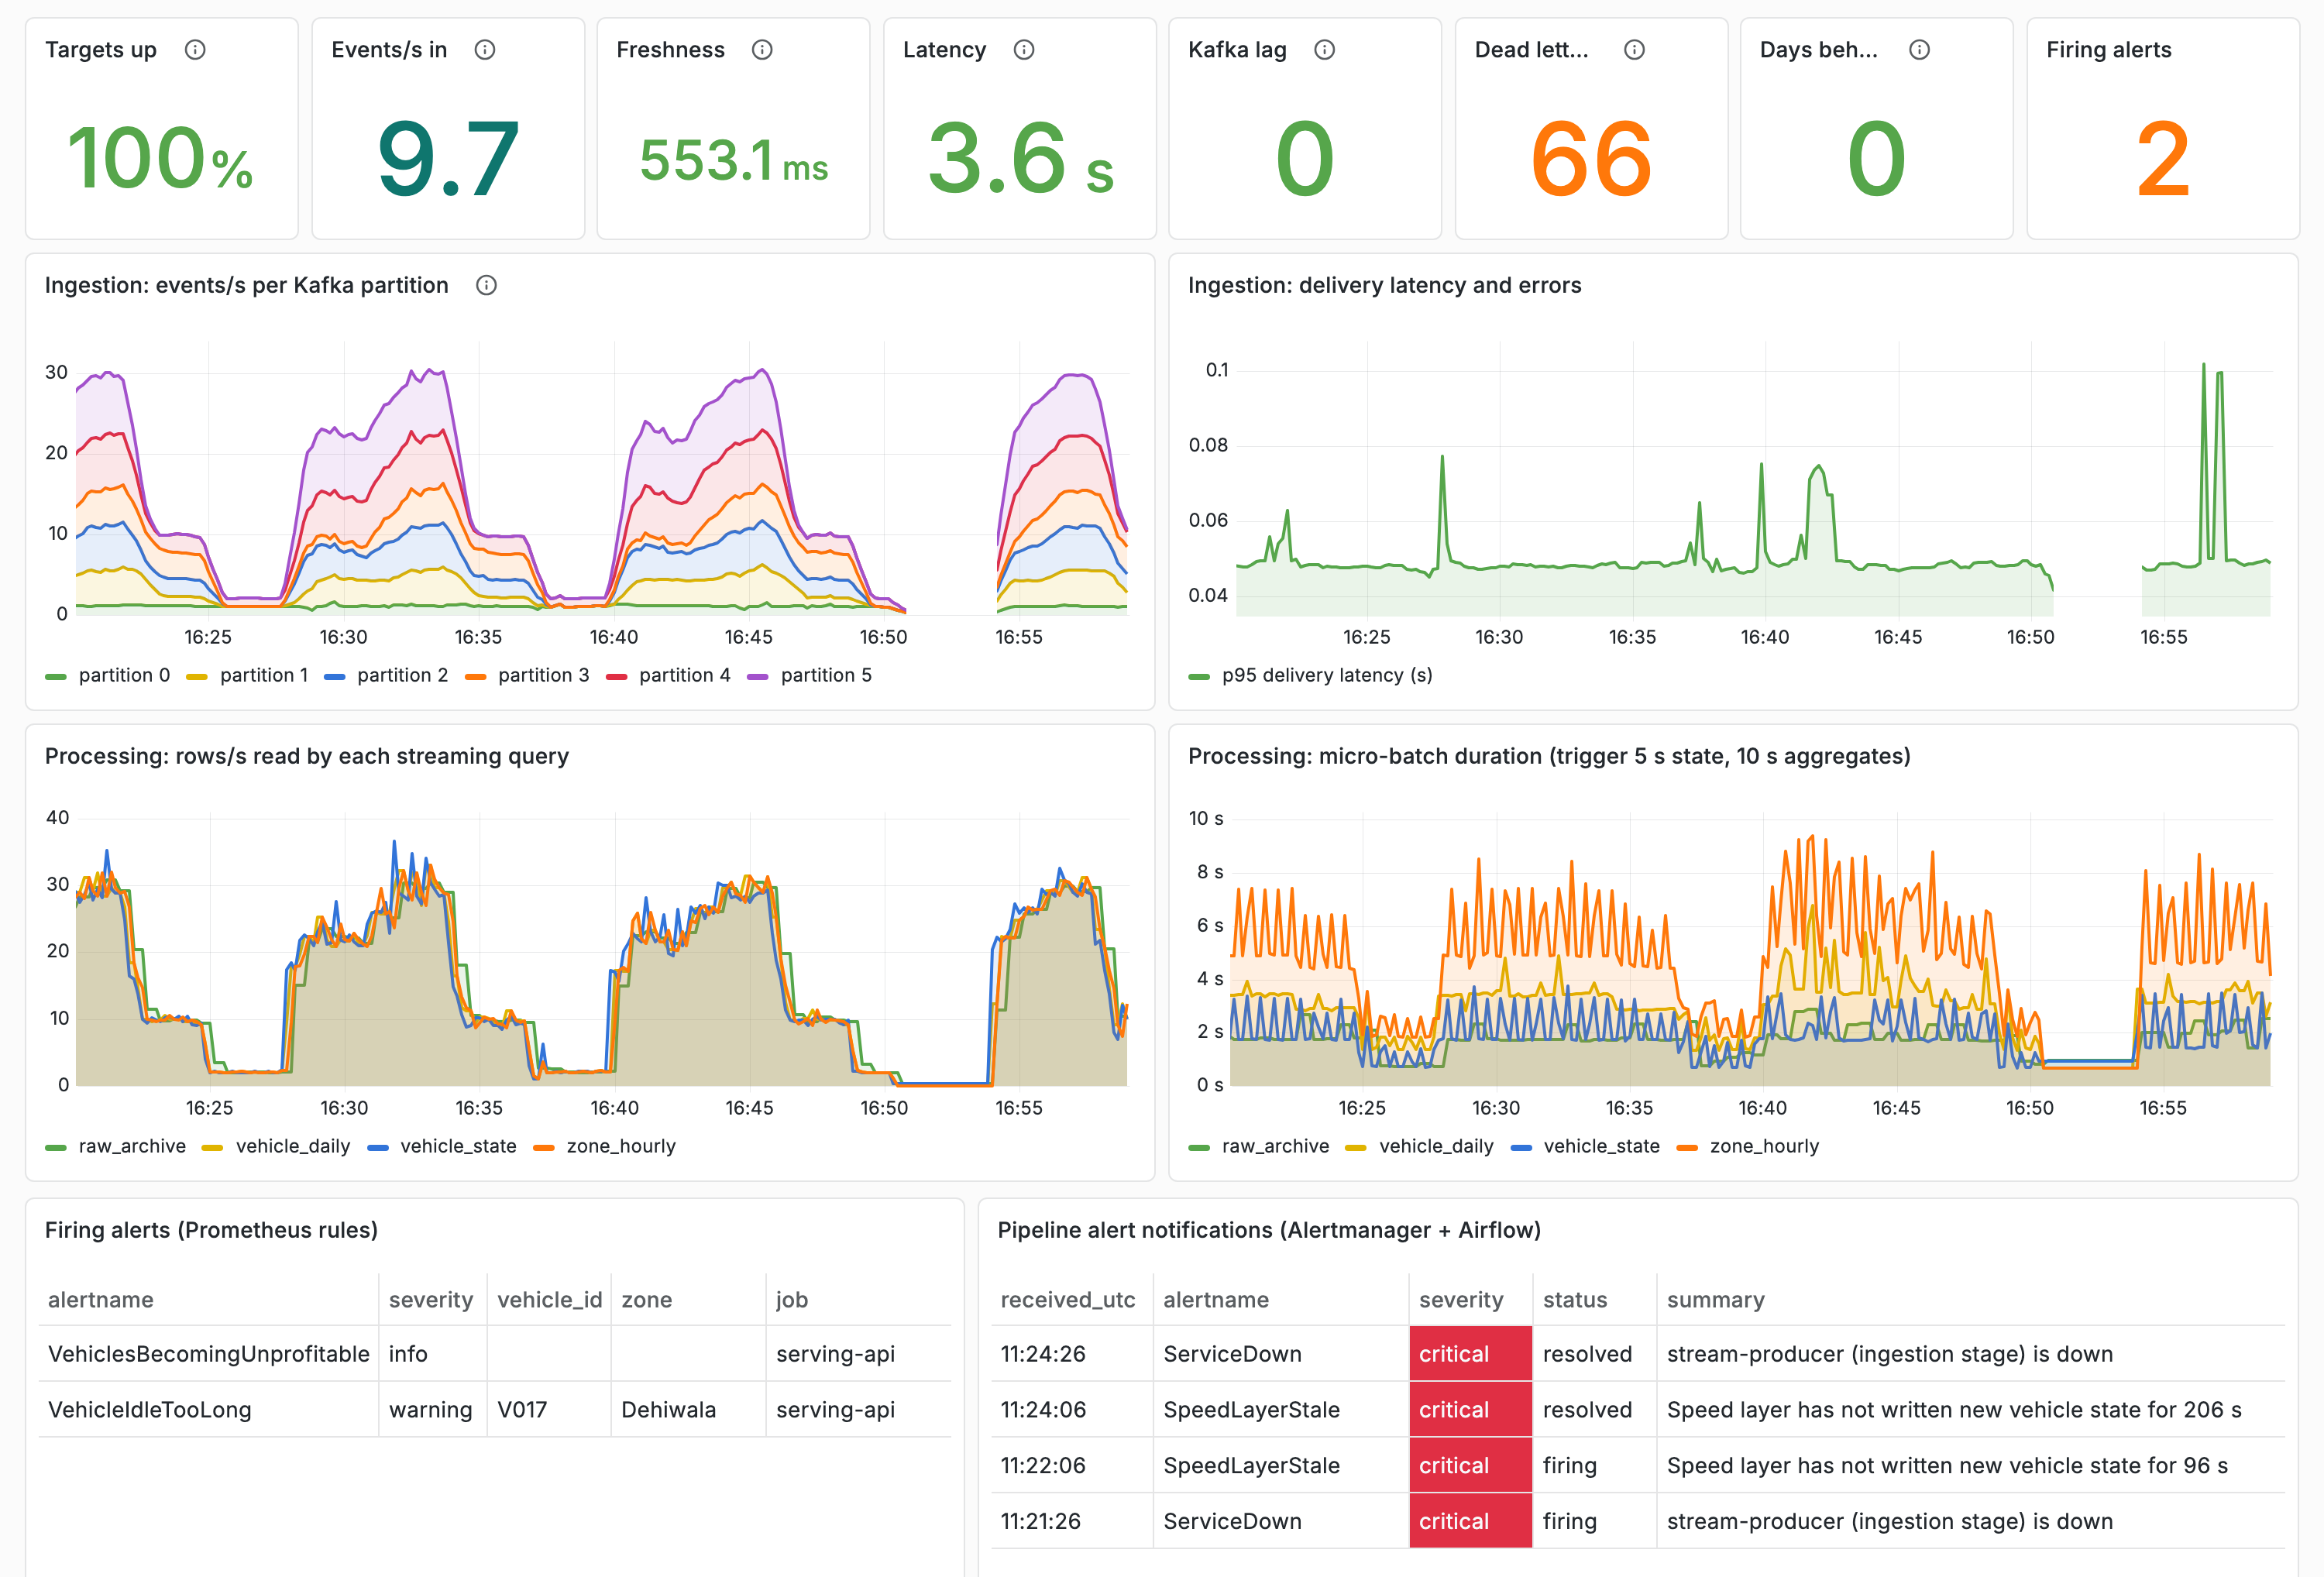
\includegraphics[width=0.92\textwidth]{figures/grafana_pipeline.png}
\caption{Grafana dashboard ``Pipeline health'' during the failure drill (top rows and alert tables). The gap
from 16:51 to 16:54 in the charts (Sri Lanka time) is the drill. The table on the right lists the alert
notifications that reached the API, with times in UTC. Lower rows (latency, lag, Airflow tasks and the run
audit trail) are not shown.}
\label{fig:health}
\end{figure}

\subsection{Performance on one laptop}
Table~\ref{tab:perf} shows speed and resource use measured during the run.

\begin{table}[!htb]
\centering\small
\caption{Speed and resource use during the run.}
\label{tab:perf}
\begin{tabularx}{\textwidth}{@{}L r@{}}
\toprule
\textbf{Measure} & \textbf{Value} \\
\midrule
Events per second into Kafka (average) & 15.8 \\
Producer delivery latency, 95th percentile & 48\,ms \\
End-to-end latency Kafka to PostgreSQL, vehicle state (average) & 2.3\,s \\
End-to-end latency, oldest record in a vehicle-state batch (maximum) & 8.2\,s \\
End-to-end latency, zone by hour windows (average) & 5.3\,s \\
Micro-batch duration: vehicle state and zone by hour (average) & 2.0\,s and 4.9\,s \\
Largest Kafka lag of any streaming query & 0 offsets \\
Spark batch job for one simulated day (average) & 20\,s \\
\midrule
\multicolumn{2}{@{}p{\dimexpr\textwidth\relax}@{}}{\raggedright\textbf{Batch job steps (average):} spark start 4\,s, validate expenses 1\,s, clean telemetry 8\,s, join and profitability 3\,s, write curated parquet 3\,s, publish postgres 1\,s} \\
\multicolumn{2}{@{}p{\dimexpr\textwidth\relax}@{}}{\raggedright\textbf{Memory per container:} airflow 438, alertmanager 43, api 41, batch-producer 10, grafana 232, kafka 77, postgres 64, prometheus 132, spark-streaming 786, statsd-exporter 36, stream-producer 37 (MiB, total 1.9\,GiB)} \\
\bottomrule
\end{tabularx}
\end{table}


\subsection{Testing}
The project has 39 automated tests (\code{pytest}), which run in their own Docker image. They cover the
simulated clock, the zone lookup, the fleet model, the cost file and its manifest, the idle-streak logic,
every validation rule, the zone metrics and profit rules in Spark, and a full batch-layer run on a small
synthetic day with known answers. One test checks that the Spark profit rules give the same answer as the
Python rules, which protects the two Lambda code paths from drifting apart. All 39 tests pass.
